% Student paper — English, typeset text, graphs/spectra as CIE clips. Compiler: XeLaTeX.
\documentclass[10pt,a4paper]{article}

\usepackage[margin=16mm,headheight=13pt,headsep=5pt,footskip=9mm]{geometry}
\usepackage{fontspec}
\usepackage[version=4]{mhchem}
\usepackage{chemfig}
\usepackage{graphicx}
\usepackage{xcolor}
\usepackage{booktabs}
\usepackage{array}
\usepackage{enumitem}
\usepackage{needspace}
\usepackage{fancyhdr}
\usepackage{amsmath,amssymb}
\usepackage{pgffor}

\raggedbottom
\setlist[enumerate]{leftmargin=1.5em,itemsep=0.12em,topsep=0.15em,parsep=0pt}
\setlist[itemize]{leftmargin=1.3em,itemsep=0.08em}

\pagestyle{fancy}
\fancyhf{}
\fancyhead[L]{\small \homeworktitle}
\fancyhead[R]{\small \homeworkmarks}
\fancyfoot[C]{\thepage}
\renewcommand{\headrulewidth}{0.3pt}

\newcommand{\homeworktitle}{Chemistry homework}
\newcommand{\homeworkmarks}{}
\newcommand{\sethomework}[2]{%
  \renewcommand{\homeworktitle}{#1}%
  \renewcommand{\homeworkmarks}{#2}%
}

\newcommand{\answerlines}[1]{%
  \par\vspace{0.08em}%
  \foreach \n in {1,...,#1}{\noindent\rule{\linewidth}{0.2pt}\\[0.62em]}%
}

\graphicspath{{images/}}
\DeclareGraphicsExtensions{.png,.jpg,.jpeg,.pdf}

\setlength{\parindent}{0pt}
\setlength{\parskip}{0.10em}
\setlength{\abovedisplayskip}{0.25em}
\setlength{\belowdisplayskip}{0.25em}

\newcommand{\qhead}[2]{%
  \par\vspace{0.28em}%
  \Needspace{4.2em}%
  \noindent{\small\textbf{#1}}\hfill{\small[#2]}\par\vspace{0.08em}%
}

\newcommand{\optline}[1]{%
  \par\vspace{0.06em}{\small #1}\par
}

\begin{document}
\sethomework{AS Chemistry --- Topic 1 Atomic Structure (Exam)}{34 marks}

\begin{center}
{\large\bfseries AS Chemistry --- Topic 1 Atomic Structure (Exam)}\\[0.12em]
{\small CIE 9701 AS Chemistry · 34 marks · about 40--45 minutes}
\end{center}

{\small Topic 1: particles and isotopes, mass spectrometry, electronic configuration / orbitals, and ionisation energy.
Answer in English. Section A is Paper 1 style (1 mark each). Section B is written; show working and give the usual CIE reasons (nuclear charge, radius, shielding, spin-pair repulsion) where asked. A Periodic Table may be used.}

\vspace{0.15em}
{\small
\begin{tabular}{@{}llr@{}}
\toprule
\textbf{Section} & \textbf{Content} & \textbf{Marks} \\
\midrule
A & Multiple choice & 13 \\
B1 & Iron mass spectrum, particles and ionisation energy & 11 \\
B2 & Electronic configuration, orbitals, ionisation energy and radii & 10 \\
\midrule
 & \textbf{Total} & \textbf{34} \\
\bottomrule
\end{tabular}}

\vspace{0.30em}
{\large\bfseries Section A --- Multiple-choice questions (13 marks)}\par

\Needspace{14em}
\qhead{A1.}{1}
{\small The table shows the numbers of protons, neutrons and electrons in four different particles, W, X, Y and Z.}

\vspace{0.10em}
\centering
{\small
\begin{tabular}{cccc}
\toprule
particle & number of protons & number of neutrons & number of electrons \\
\midrule
W & 32 & 40 & 32 \\
X & 32 & 40 & 34 \\
Y & 32 & 42 & 32 \\
Z & 34 & 40 & 34 \\
\bottomrule
\end{tabular}}
\par\raggedright

\vspace{0.10em}
{\small Which pair represents the atoms of two isotopes of the same element?}
\vspace{0.06em}
{\small
\begin{tabular}{@{}p{0.46\linewidth}p{0.46\linewidth}@{}}
\textbf{A} W and Y & \textbf{B} W and Z \\[0.12em]
\textbf{C} X and Y & \textbf{D} X and Z
\end{tabular}}
\par

\qhead{A2.}{1}
{\small An ion with a charge of 2-- contains 10 electrons and 14 neutrons.}

{\small What is its nucleon number?}
\vspace{0.06em}
{\small
\begin{tabular}{@{}p{0.22\linewidth}p{0.22\linewidth}p{0.22\linewidth}p{0.22\linewidth}@{}}
\textbf{A} 14 & \textbf{B} 22 & \textbf{C} 24 & \textbf{D} 26
\end{tabular}}
\par

\Needspace{12em}
\qhead{A3.}{1}
{\small What is the total number of protons, neutrons and electrons present in an ammonium ion with a relative formula mass of 21?}

\vspace{0.10em}
\centering
{\small
\begin{tabular}{cccc}
\toprule
 & number of protons & number of neutrons & number of electrons \\
\midrule
\textbf{A} & 11 & 10 & 10 \\
\textbf{B} & 10 & 11 & 11 \\
\textbf{C} & 10 & 11 & 10 \\
\textbf{D} & 11 & 10 & 11 \\
\bottomrule
\end{tabular}}
\par\raggedright

\Needspace{18em}
\qhead{A4.}{1}
{\small A helium ion contains two protons, two neutrons and one electron.}

{\small This helium ion and a proton are passed separately through a uniform electric field.}

{\small The particles are travelling at the same velocity.}

{\small Which arrow describes the path of each particle?}

\vspace{0.08em}
\begin{center}

\includegraphics[width=0.58\linewidth,keepaspectratio]{fig-a4-field.png}
\end{center}

\vspace{0.08em}
\centering
{\small
\begin{tabular}{ccc}
\toprule
 & helium ion & proton \\
\midrule
\textbf{A} & 1 & 2 \\
\textbf{B} & 2 & 1 \\
\textbf{C} & 4 & 5 \\
\textbf{D} & 5 & 4 \\
\bottomrule
\end{tabular}}
\par\raggedright

\qhead{A5.}{1}
{\small A sample of magnesium contains the isotopes \ce{^{24}Mg}, \ce{^{25}Mg} and \ce{^{26}Mg} only.}

{\small The percentage abundance of \ce{^{25}Mg} and \ce{^{26}Mg} is the same.}

{\small The relative atomic mass of magnesium in the sample is 24.3.}

{\small What is the percentage abundance of \ce{^{24}Mg}?}
\vspace{0.06em}
{\small
\begin{tabular}{@{}p{0.22\linewidth}p{0.22\linewidth}p{0.22\linewidth}p{0.22\linewidth}@{}}
\textbf{A} 10\% & \textbf{B} 20\% & \textbf{C} 60\% & \textbf{D} 80\%
\end{tabular}}
\par

\qhead{A6.}{1}
{\small Which isolated gaseous atom has a total of five electrons occupying spherically shaped orbitals?}
\vspace{0.06em}
{\small
\begin{tabular}{@{}p{0.46\linewidth}p{0.46\linewidth}@{}}
\textbf{A} sodium & \textbf{B} fluorine \\[0.12em]
\textbf{C} boron & \textbf{D} potassium
\end{tabular}}
\par

\Needspace{16em}
\qhead{A7.}{1}
{\small What is the electrons in boxes notation for the \ce{Fe^{3+}} ion?}

\vspace{0.08em}
\begin{center}
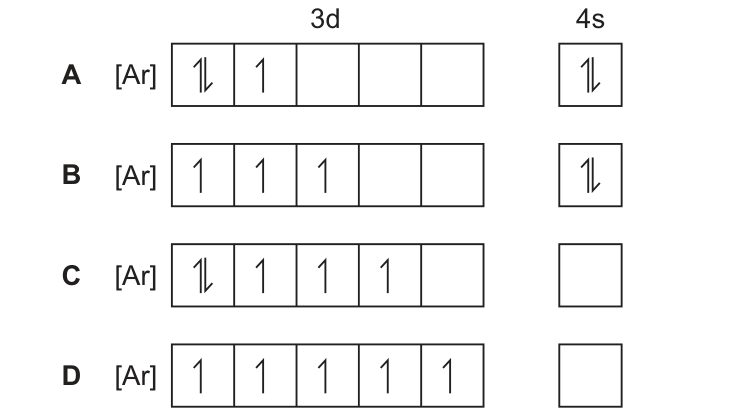
\includegraphics[width=0.78\linewidth,keepaspectratio]{fig-a7-boxes.png}
\end{center}

\qhead{A8.}{1}
{\small Which atom has more unpaired electrons than paired electrons in orbitals of principal quantum number 2?}
\vspace{0.06em}
{\small
\begin{tabular}{@{}p{0.46\linewidth}p{0.46\linewidth}@{}}
\textbf{A} carbon & \textbf{B} nitrogen \\[0.12em]
\textbf{C} oxygen & \textbf{D} fluorine
\end{tabular}}
\par

\Needspace{12em}
\qhead{A9.}{1}
{\small Why is the first ionisation energy of oxygen less than that of nitrogen?}
\begin{enumerate}[label=\textbf{\Alph*}, leftmargin=1.7em, itemsep=0.08em]
\item The nitrogen atom has its outer electron in a different subshell.
\item The nuclear charge on the oxygen atom is greater than that on the nitrogen atom.
\item The oxygen atom has a pair of electrons in one p orbital that repel one another.
\item There is more shielding in an oxygen atom.
\end{enumerate}

\Needspace{16em}
\qhead{A10.}{1}
{\small Equations involving four enthalpy changes are shown.}

\vspace{0.08em}
\centering
{\small
\begin{tabular}{ll}
\ce{Na(g) -> Na+(g) + e-} & $\Delta H = W$ \\[0.15em]
\ce{Na(g) -> Na^{2+}(g) + 2e-} & $\Delta H = X$ \\[0.15em]
\ce{Na(s) -> Na(g)} & $\Delta H = Y$ \\[0.15em]
\ce{Na(s) -> Na^{2+}(g) + 2e-} & $\Delta H = Z$
\end{tabular}}
\par\raggedright

\vspace{0.10em}
{\small Which equation represents the second ionisation energy of sodium?}
\vspace{0.06em}
{\small
\begin{tabular}{@{}p{0.46\linewidth}p{0.46\linewidth}@{}}
\textbf{A} $X$ & \textbf{B} $X + Y - W$ \\[0.12em]
\textbf{C} $X - W$ & \textbf{D} $Z - W$
\end{tabular}}
\par

\Needspace{12em}
\qhead{A11.}{1}
{\small The first seven ionisation energies of an element between lithium and neon in the Periodic Table are shown.}

\vspace{0.08em}
\centering
{\small 1310 \quad 3390 \quad 5320 \quad 7450 \quad 11000 \quad 13300 \quad 71000 \quad kJ\,mol$^{-1}$}
\par\raggedright

\vspace{0.10em}
{\small What is the outer electronic configuration of the element?}
\vspace{0.06em}
{\small
\begin{tabular}{@{}p{0.46\linewidth}p{0.46\linewidth}@{}}
\textbf{A} \ce{2s^2} & \textbf{B} \ce{2s^2 2p^1} \\[0.12em]
\textbf{C} \ce{2s^2 2p^4} & \textbf{D} \ce{2s^2 2p^6}
\end{tabular}}
\par

\Needspace{22em}
\qhead{A12.}{1}
{\small The graph shows the variation of the first ionisation energy with proton number for some elements.}

{\small The letters used are \textbf{not} the actual symbols for the elements.}

\vspace{0.08em}
\begin{center}
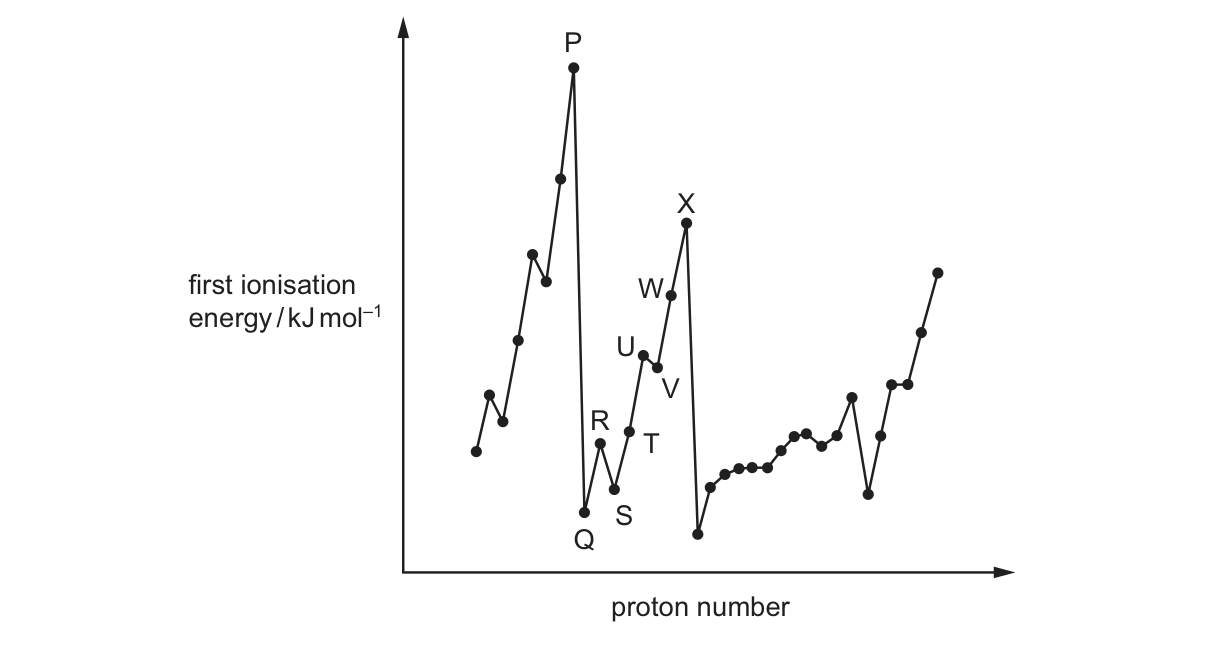
\includegraphics[width=0.86\linewidth,keepaspectratio]{fig-a12-ie.png}
\end{center}

{\small Which statement about the elements is correct?}
\begin{enumerate}[label=\textbf{\Alph*}, leftmargin=1.7em, itemsep=0.08em]
\item P and X are in the same period in the Periodic Table.
\item The general increase from Q to X is due to increasing atomic radius.
\item The small decrease from R to S is due to decreased shielding.
\item The small decrease from U to V is due to repulsion between paired electrons.
\end{enumerate}

\Needspace{14em}
\qhead{A13.}{1}
{\small Which statements about first ionisation energies are correct?}
\begin{enumerate}[label=\arabic*., leftmargin=1.6em, itemsep=0.06em]
\item They are always endothermic.
\item They decrease down Group 2.
\item They decrease across Period 3.
\end{enumerate}
{\small Which statements are correct?}
\vspace{0.08em}
\centering
{\small
\begin{tabular}{cccc}
\toprule
\textbf{A} & \textbf{B} & \textbf{C} & \textbf{D} \\
\midrule
1, 2 and 3 & 1 and 2 only & 2 and 3 only & 1 only \\
\bottomrule
\end{tabular}}
\par\raggedright

\Needspace{24em}
\vspace{0.40em}
{\large\bfseries Section B --- Structured questions (21 marks)}\par\vspace{0.12em}
{\normalsize\bfseries B1 · Iron mass spectrum, particles and ionisation energy (11 marks)}\par

{\small A sample of iron is analysed using a mass spectrometer. The mass spectrum shows three isotopes of iron are present in the sample.}

\qhead{B1(a)}{1}
{\small Define isotopes.}
\answerlines{2}

\Needspace{16em}
\qhead{B1(b)(i)}{2}
{\small Fig.~2.1 shows the mass spectrum of the sample of iron.}

\vspace{0.08em}
\begin{center}
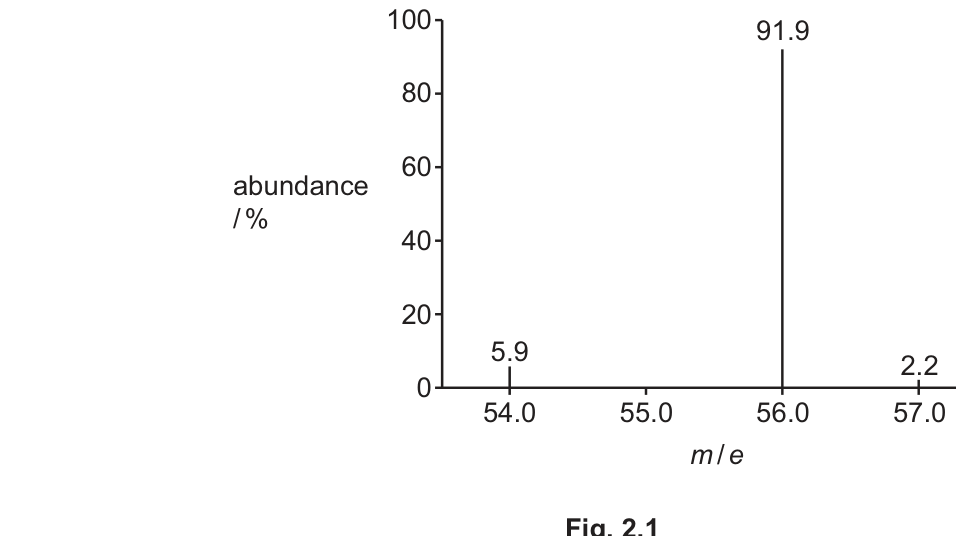
\includegraphics[width=0.78\linewidth,keepaspectratio]{fig-b1-spectrum.png}
\end{center}

{\small Use Fig.~2.1 to calculate the relative atomic mass, $A_\mathrm{r}$, of iron to one decimal place.}

{\small Show your working.}
\answerlines{3}
{\small $A_\mathrm{r}$ of iron = \underline{\hspace{3.2cm}}}

\Needspace{10em}
\qhead{B1(b)(ii)}{2}
{\small Complete Table 2.1 to show the number of protons and nucleons in one atom of \ce{^{56}Fe}.}

\vspace{0.10em}
\centering
{\small
\begin{tabular}{|p{3.4cm}|p{6.4cm}|}
\hline
particle & number of particles in one atom of \ce{^{56}Fe} \\
\hline
protons & \vspace{0.85em} \\
\hline
nucleons & \vspace{0.85em} \\
\hline
\end{tabular}}
\par\vspace{0.06em}
{\small Table 2.1}\par
\raggedright

\qhead{B1(c)}{1}
{\small Deduce the number of pairs of electrons in the shell with principal quantum number $n = 3$ in an Fe atom.}
\vspace{0.15em}
{\small number of pairs of electrons \underline{\hspace{3.2cm}}}

\qhead{B1(d)}{1}
{\small Write an equation to represent the first ionisation energy of iron.}
\answerlines{2}

\qhead{B1(e)}{4}
{\small Suggest how the value for the first ionisation energy of \ce{^{54}Fe} compares to the first ionisation energy of \ce{^{56}Fe}. Explain your answer in terms of the factors that affect ionisation energy.}
\answerlines{5}

\Needspace{22em}
\vspace{0.35em}
\Needspace{10em}
{\normalsize\bfseries B2 · Electronic configuration, orbitals, ionisation energy and radii (10 marks)}\par

{\small The chemical properties of an element are related to the electronic configuration of its atoms.}

\qhead{B2(a)(i)}{1}
{\small Give the full electronic configuration of a fluorine atom.}
\answerlines{2}

\qhead{B2(a)(ii)}{1}
{\small Deduce the number of pairs of electrons in the second energy shell, $n = 2$, of an oxygen atom.}
\vspace{0.15em}
{\small number of pairs of electrons \underline{\hspace{3.2cm}}}

\Needspace{8em}
\qhead{B2(a)(iii)}{1}
{\small Draw the shape of the highest energy orbital that contains electrons in an atom of calcium.}
\vspace{0.12em}
\fbox{\begin{minipage}[c][2.6cm][c]{3.6cm}\centering\mbox{}\end{minipage}}

\qhead{B2(b)(i)}{1}
{\small Write an equation to represent the first ionisation energy of sulfur.}
\answerlines{2}

\qhead{B2(b)(ii)}{2}
{\small Explain why the first ionisation energy of sulfur is less than the first ionisation energy of phosphorus.}
\answerlines{3}

\Needspace{12em}
\qhead{B2(b)(iii)}{4}
{\small Arrange the three species \ce{F-}, \ce{Ne} and \ce{Na+} in order of increasing radius.}

{\small Explain your answer.}

\vspace{0.25em}
\centering
{\small \underline{\hspace{2.6cm}} $<$ \underline{\hspace{2.6cm}} $<$ \underline{\hspace{2.6cm}}}\\[0.15em]
{\small smallest radius \hspace{4.8cm} largest radius}
\par\raggedright
\answerlines{4}

\end{document}
